\documentclass{article}
\usepackage{graphicx}
\usepackage[nomarkers]{endfloat}
\renewcommand{\efloatseparator}{\newpage}
\renewcommand{\listoffigures}{} % but suppress these lists
\renewcommand{\listoftables}{} % suppress these lists
\begin{document}

\begin{figure}[h!]
  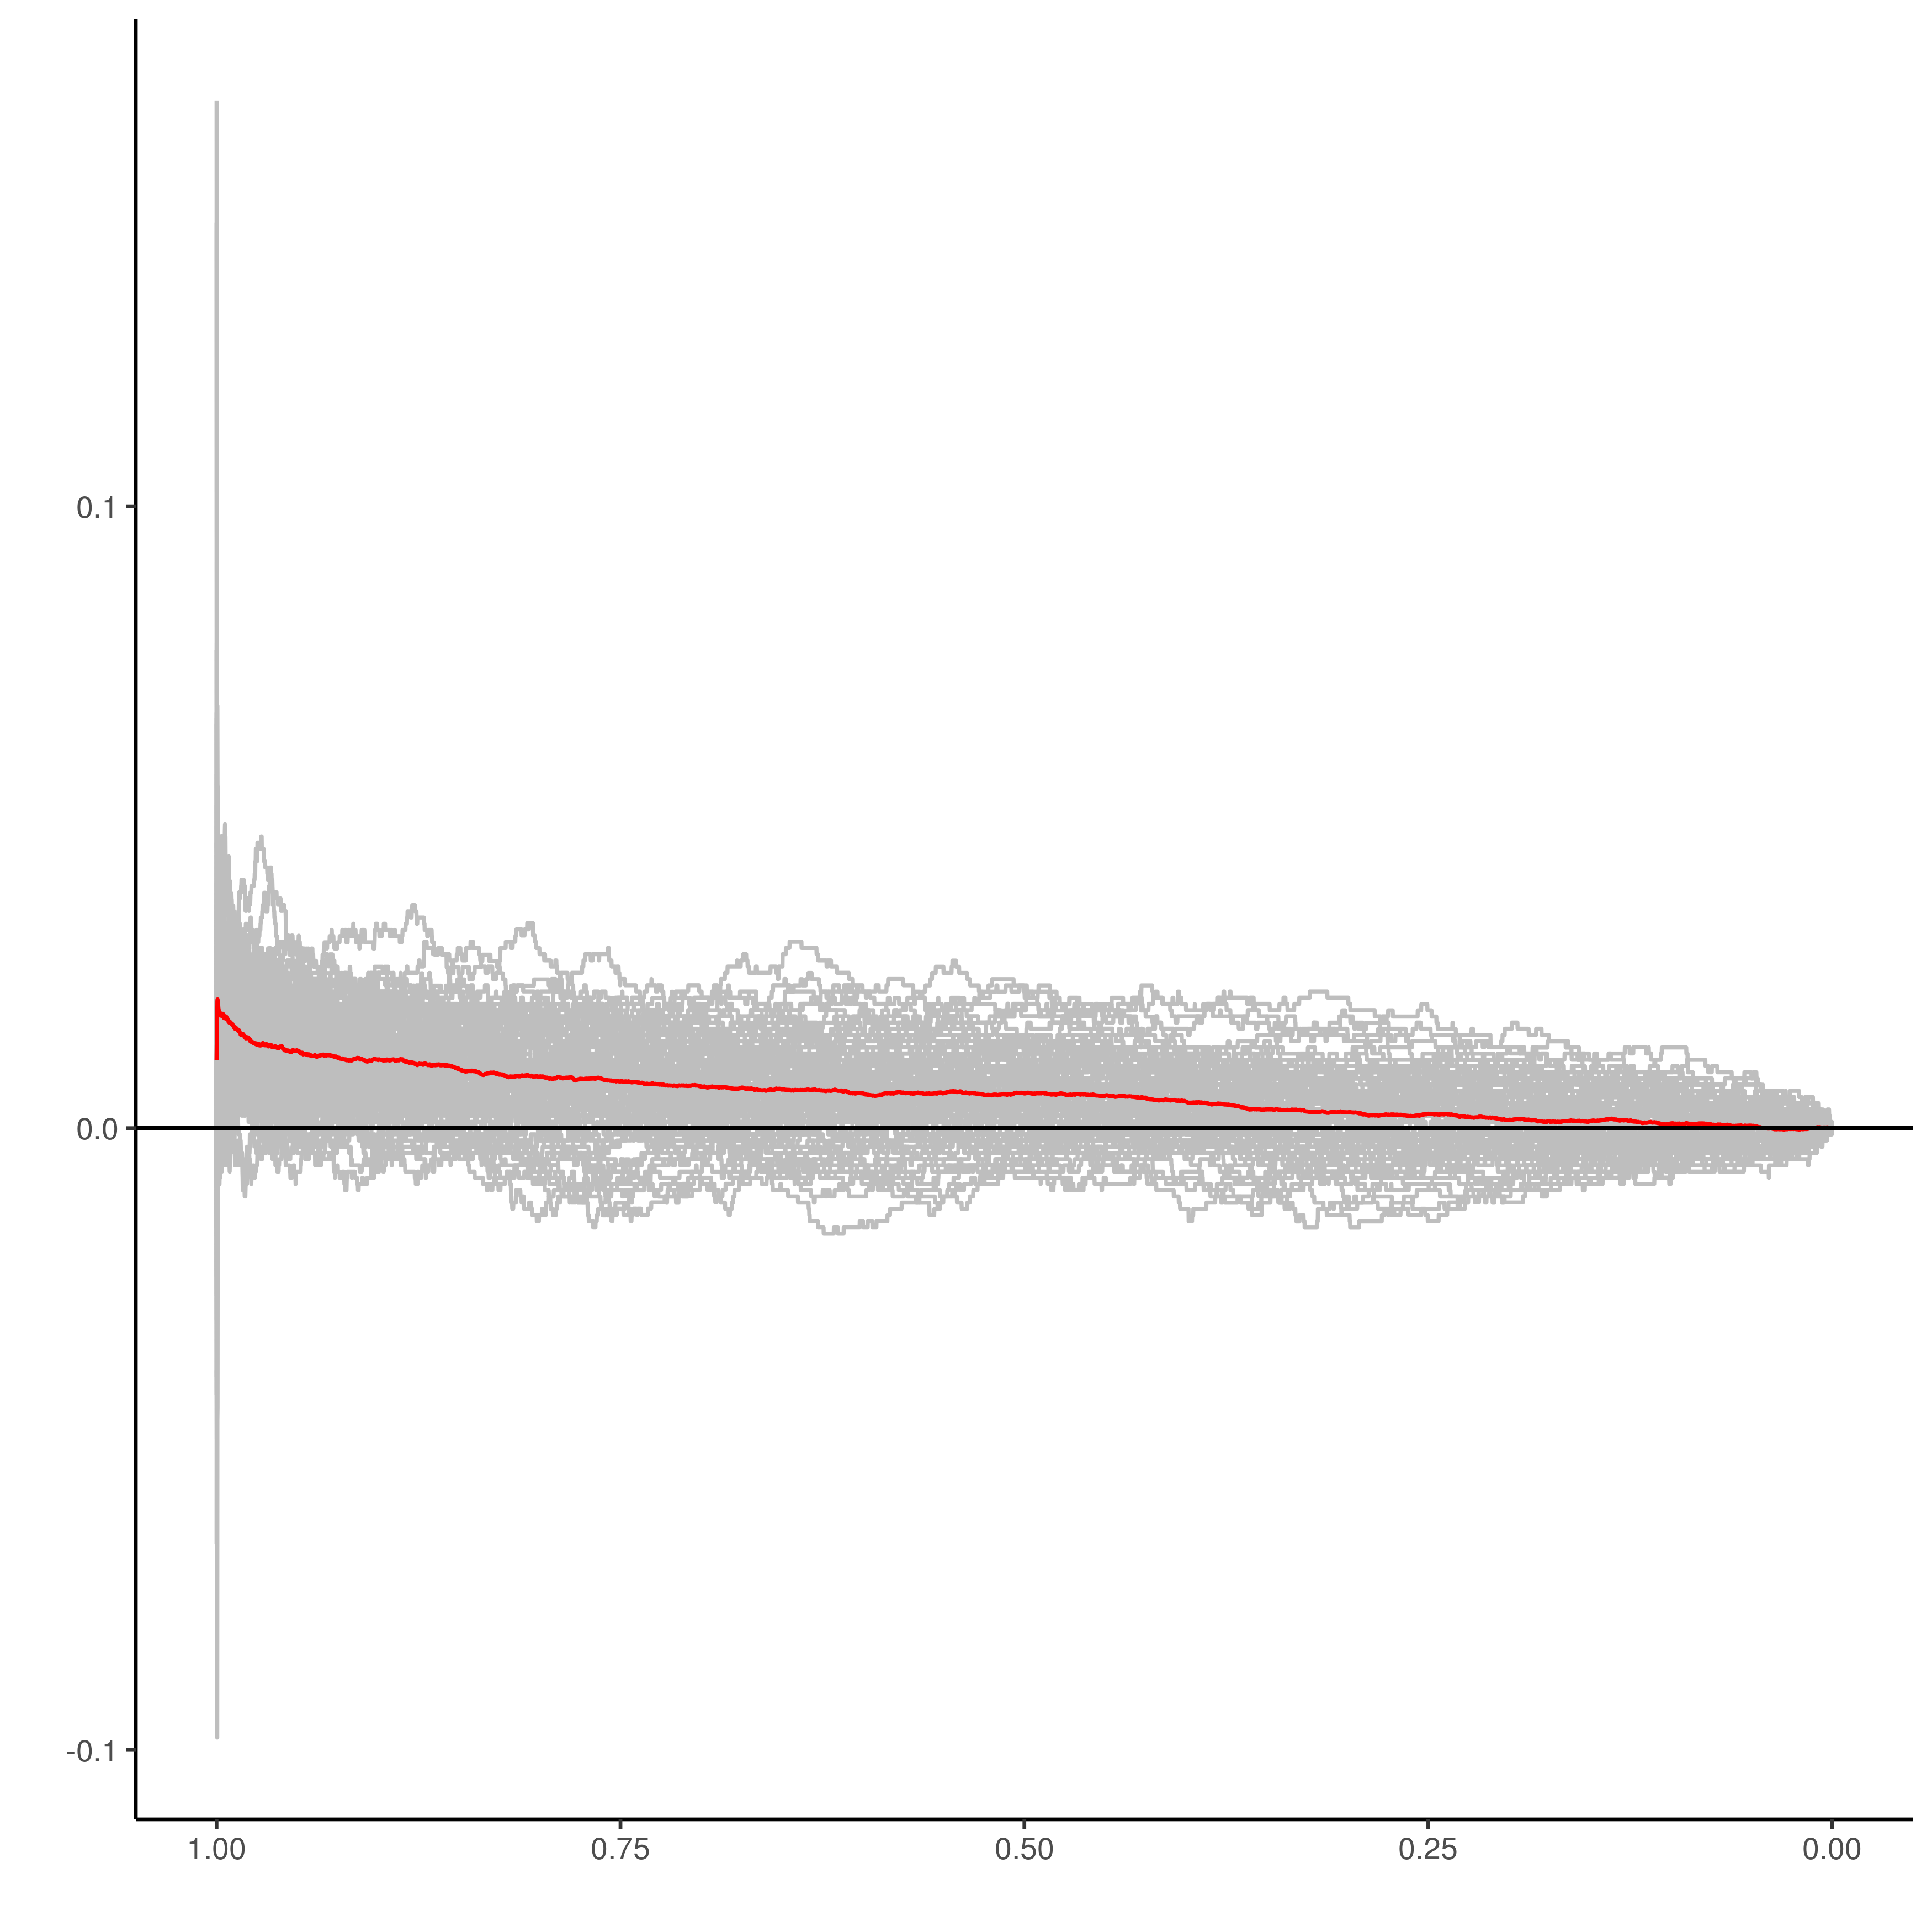
\includegraphics[width=\textwidth]{images/suppFig1.png}
  \caption{Difference in sensitivity (between the fastGWA-PGS and Bolt-LMM methods) as a function of specificity. The red line shows the mean difference over all simulations.}
\end{figure}

\begin{figure}[h!]
  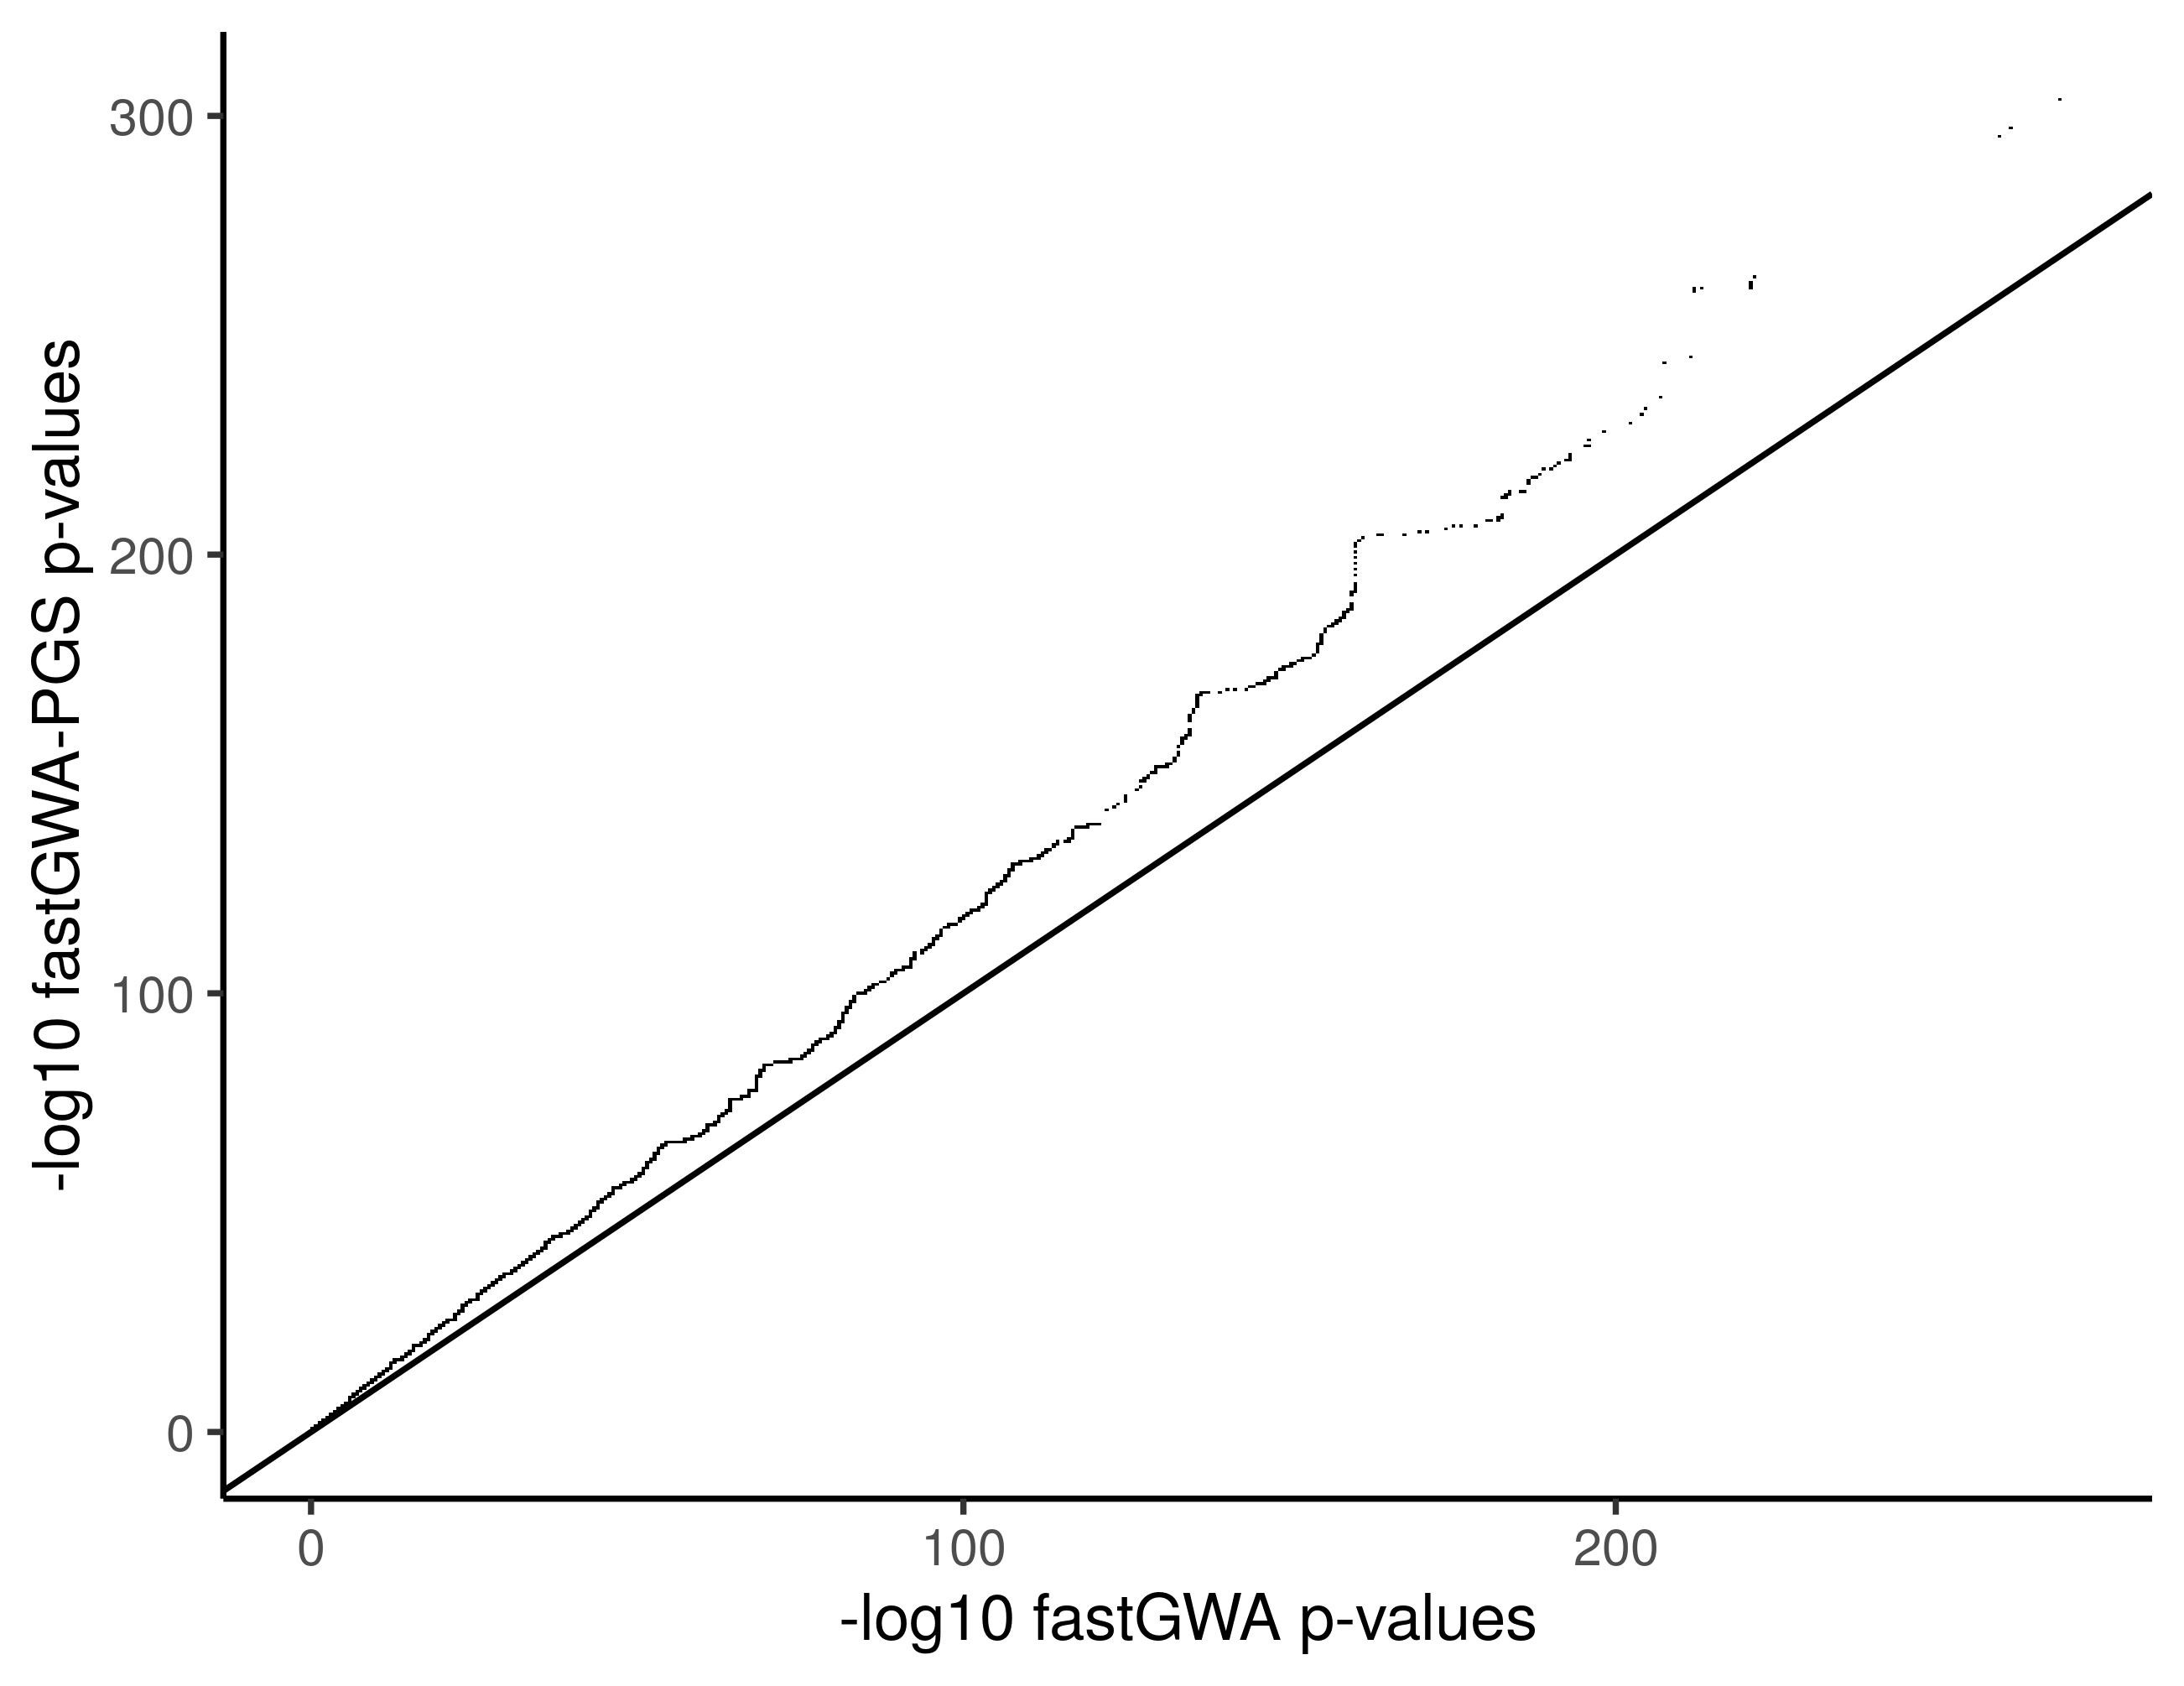
\includegraphics[width=\textwidth]{images/suppFig2.png}
  \caption{Distribution of variant significance for fastGWA-PGS (y-axis) and fastGWA (x-axis)}
\end{figure}

\begin{figure}[h!]
  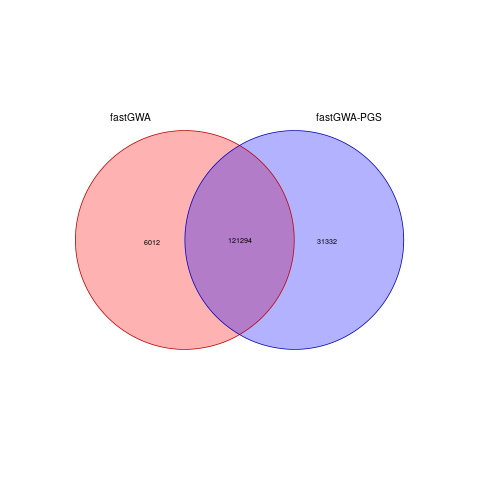
\includegraphics[width=\textwidth]{images/suppFig3.png}
  \caption{Venn diagram of significant variants identified by both FastGWA and fastGWA-PGS }
\end{figure}

\begin{figure}[h!]
  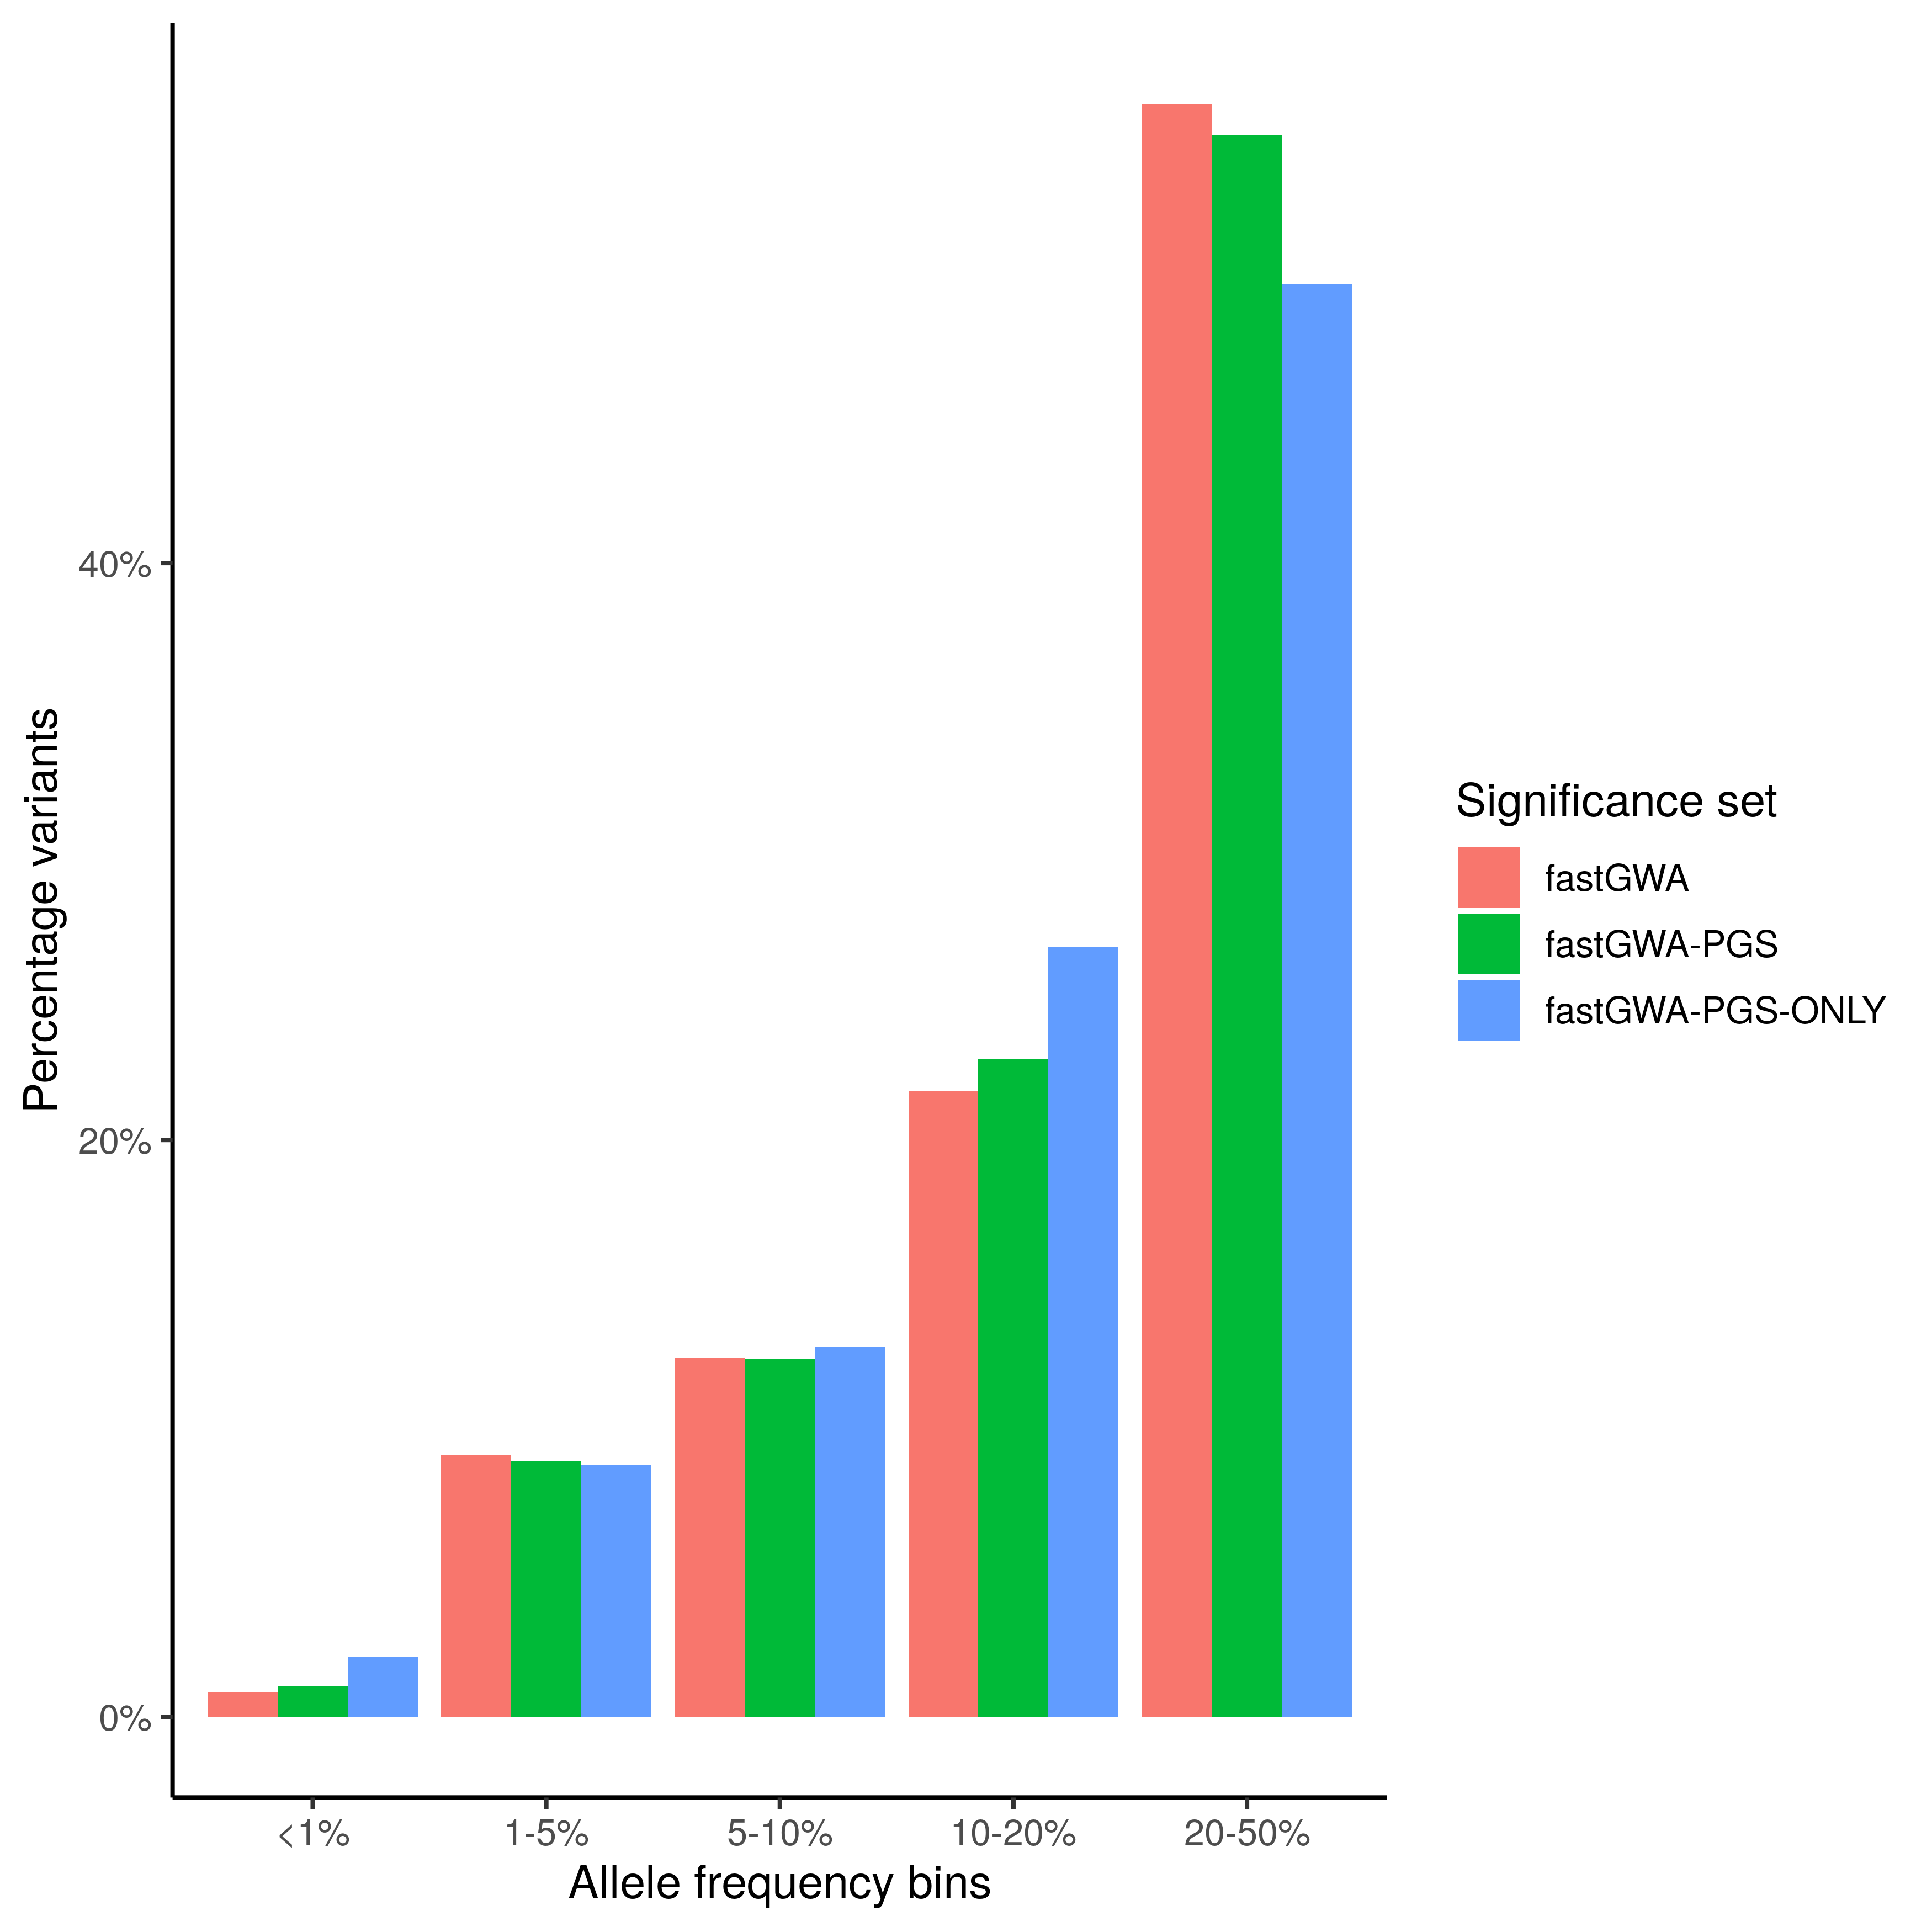
\includegraphics[width=\textwidth]{images/suppFig4.png}
  \caption{Minor allele frequency of significant variants identified by the fastGWA method (red), MAF of variants identified by fastGWA-PGS (green) and MAF of variants identified by the fastGWA-PGS method but not fastGWA (blue).}
\end{figure}

\begin{figure}[h!]
  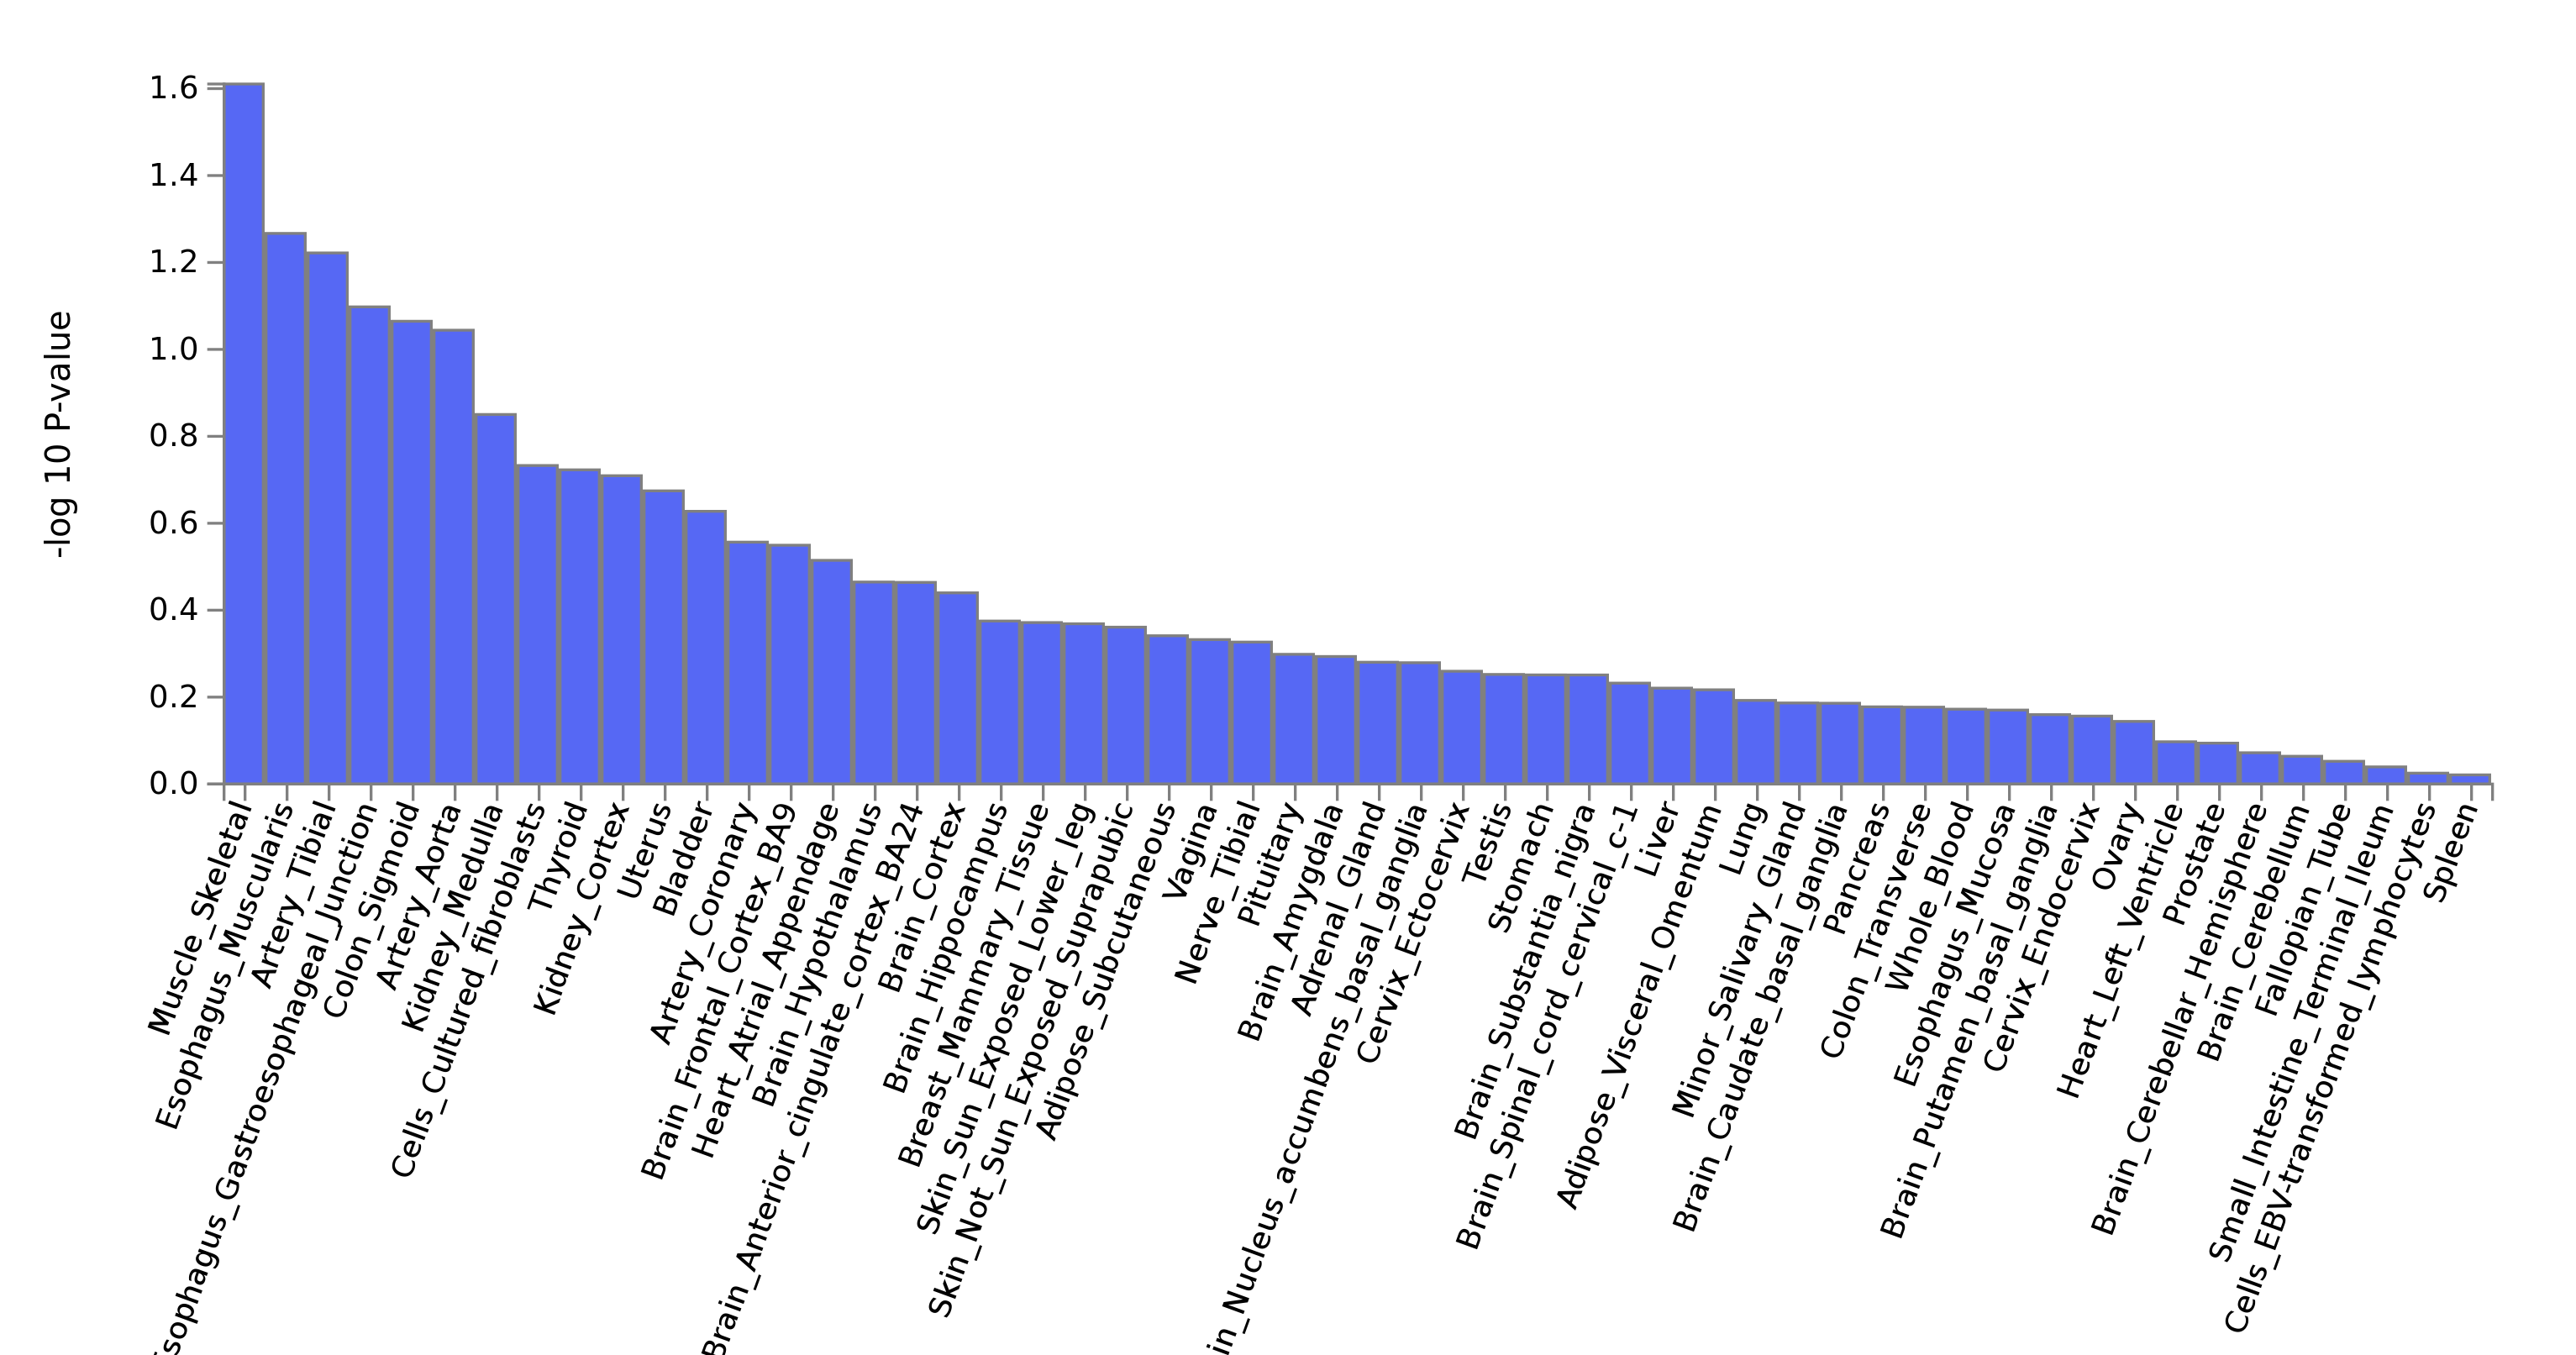
\includegraphics[width=\textwidth]{images/suppFig5.png}
  \caption{Gene-property analysis for issue specificity PGS-Only variants}
\end{figure}

\begin{figure}[h!]
  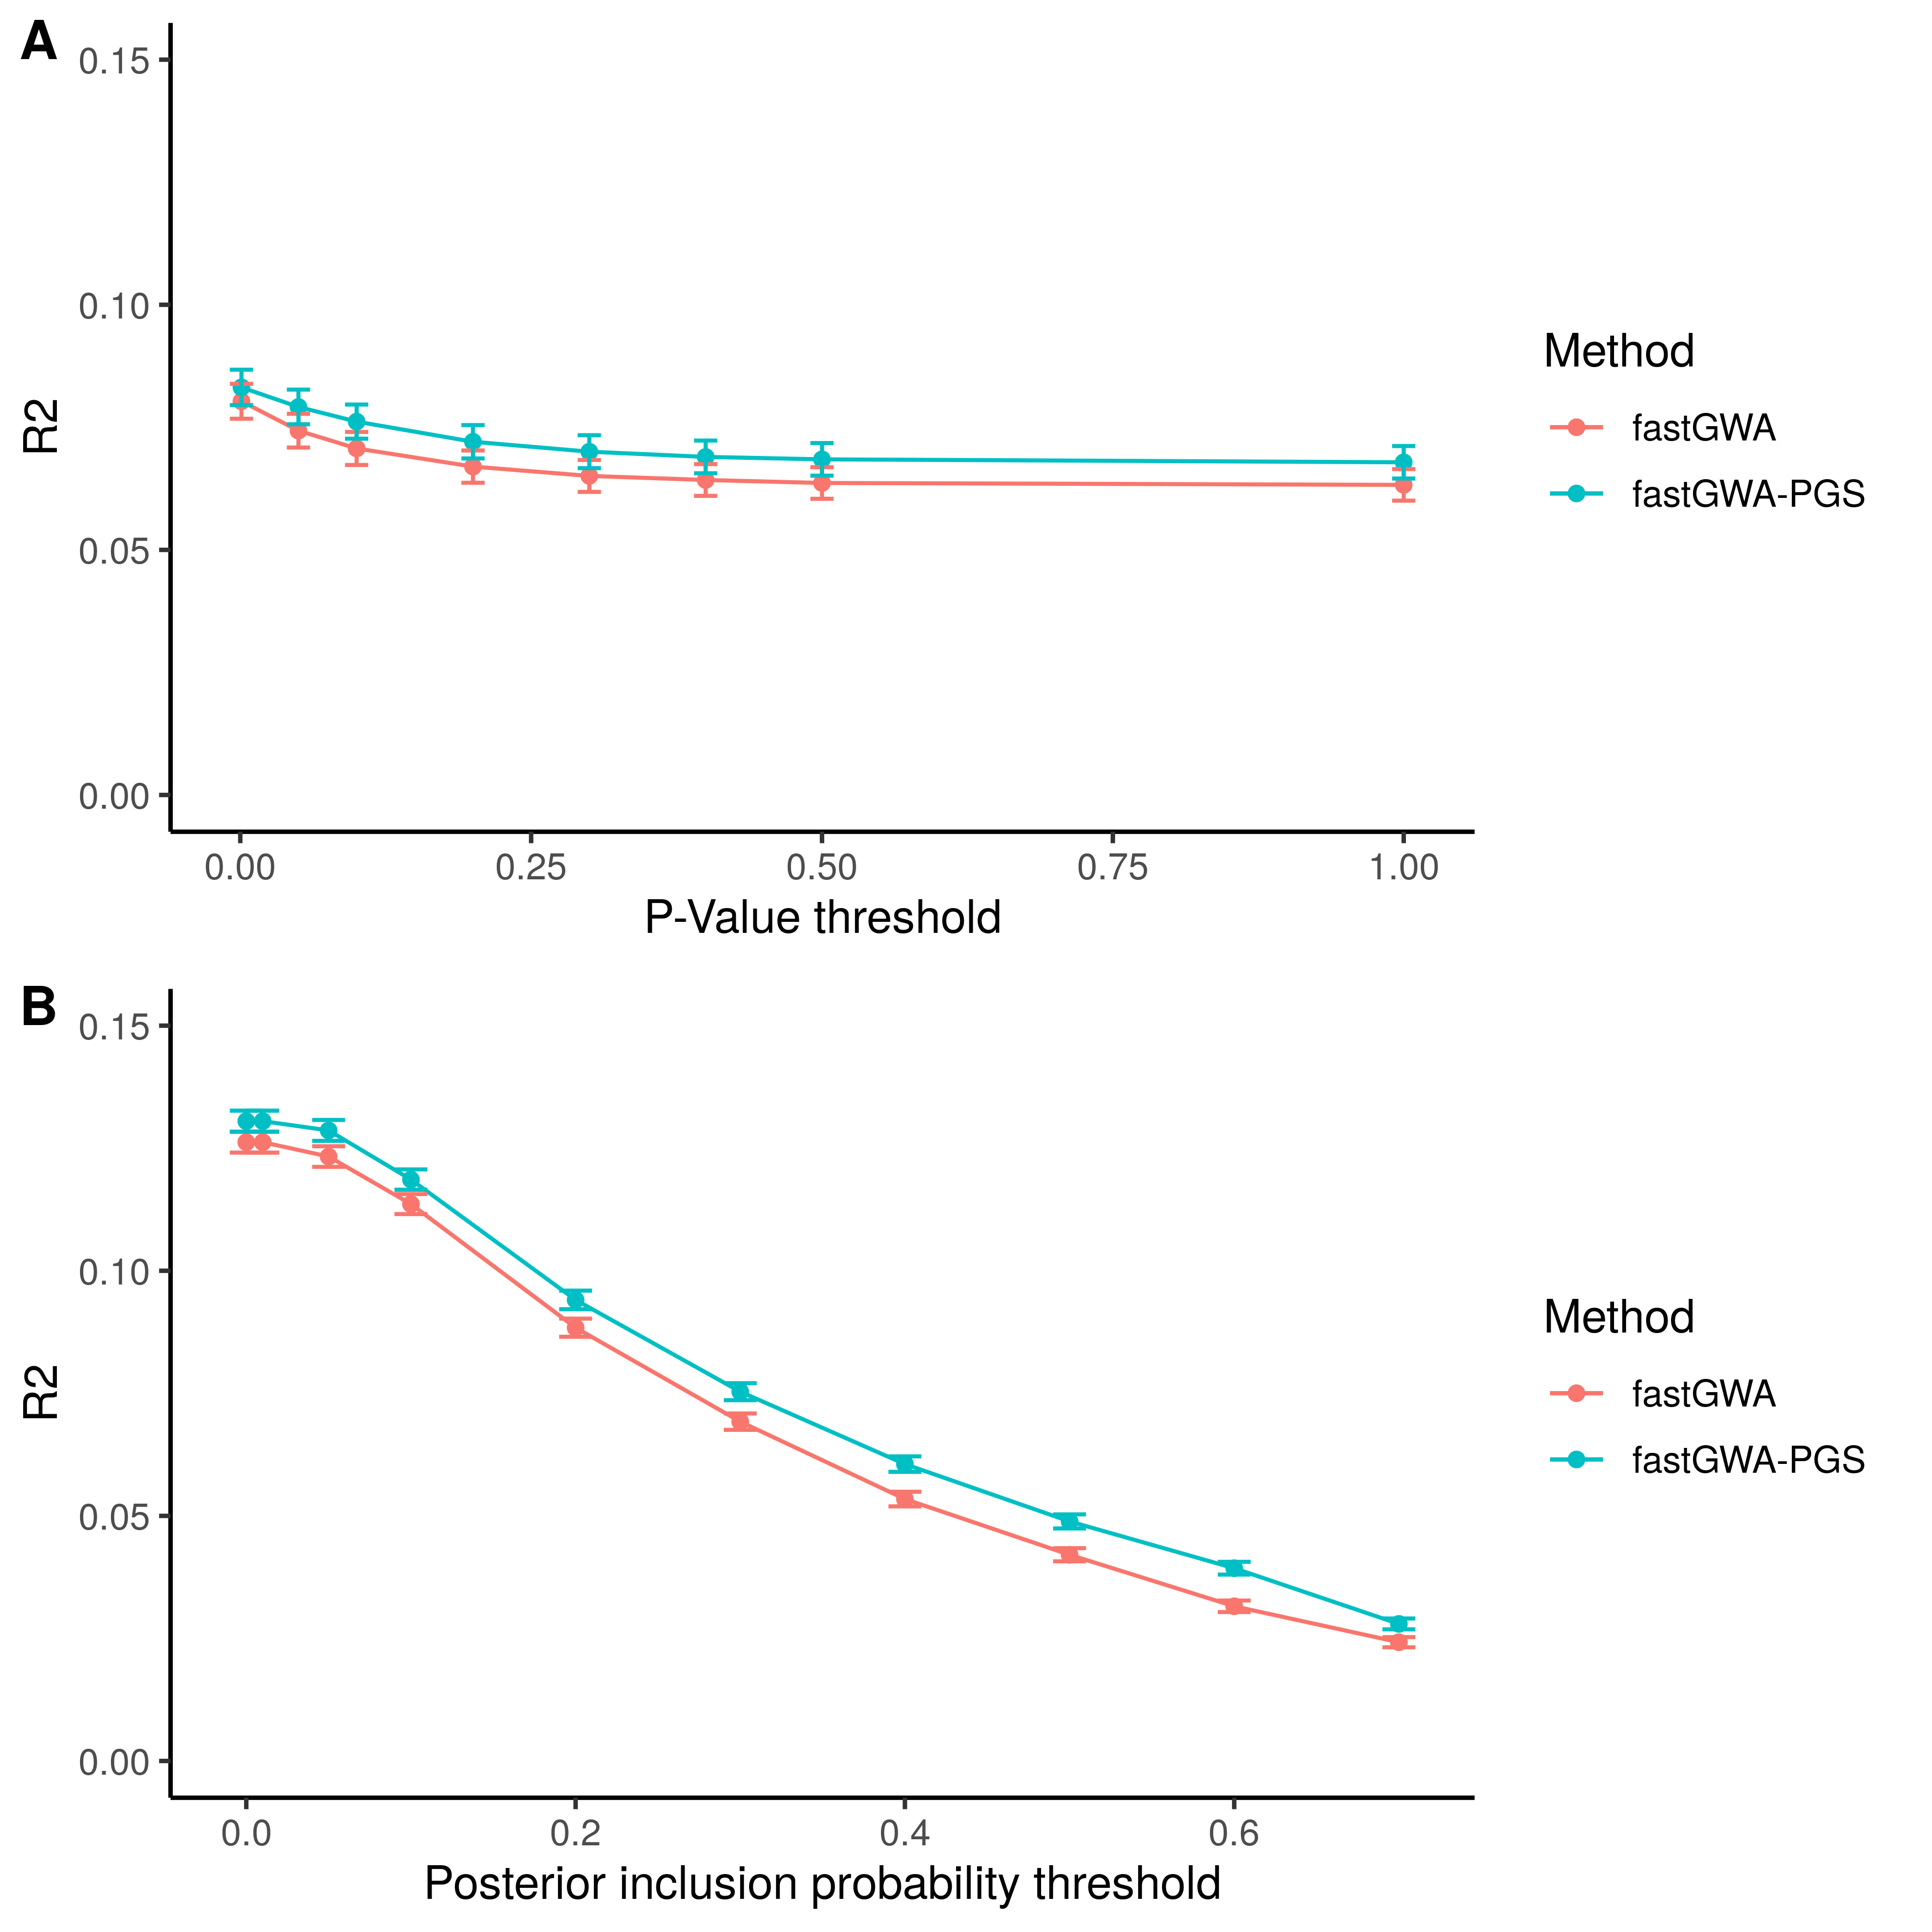
\includegraphics[width=\textwidth]{images/suppFig6.png}
  \caption{P+T prediction (A) across range of p value thresholds for each method Bayesian inference prediction (B) across PIP scores. Summary statistics are calculated on the 20\% training data}
\end{figure}

\begin{figure}[h!]
  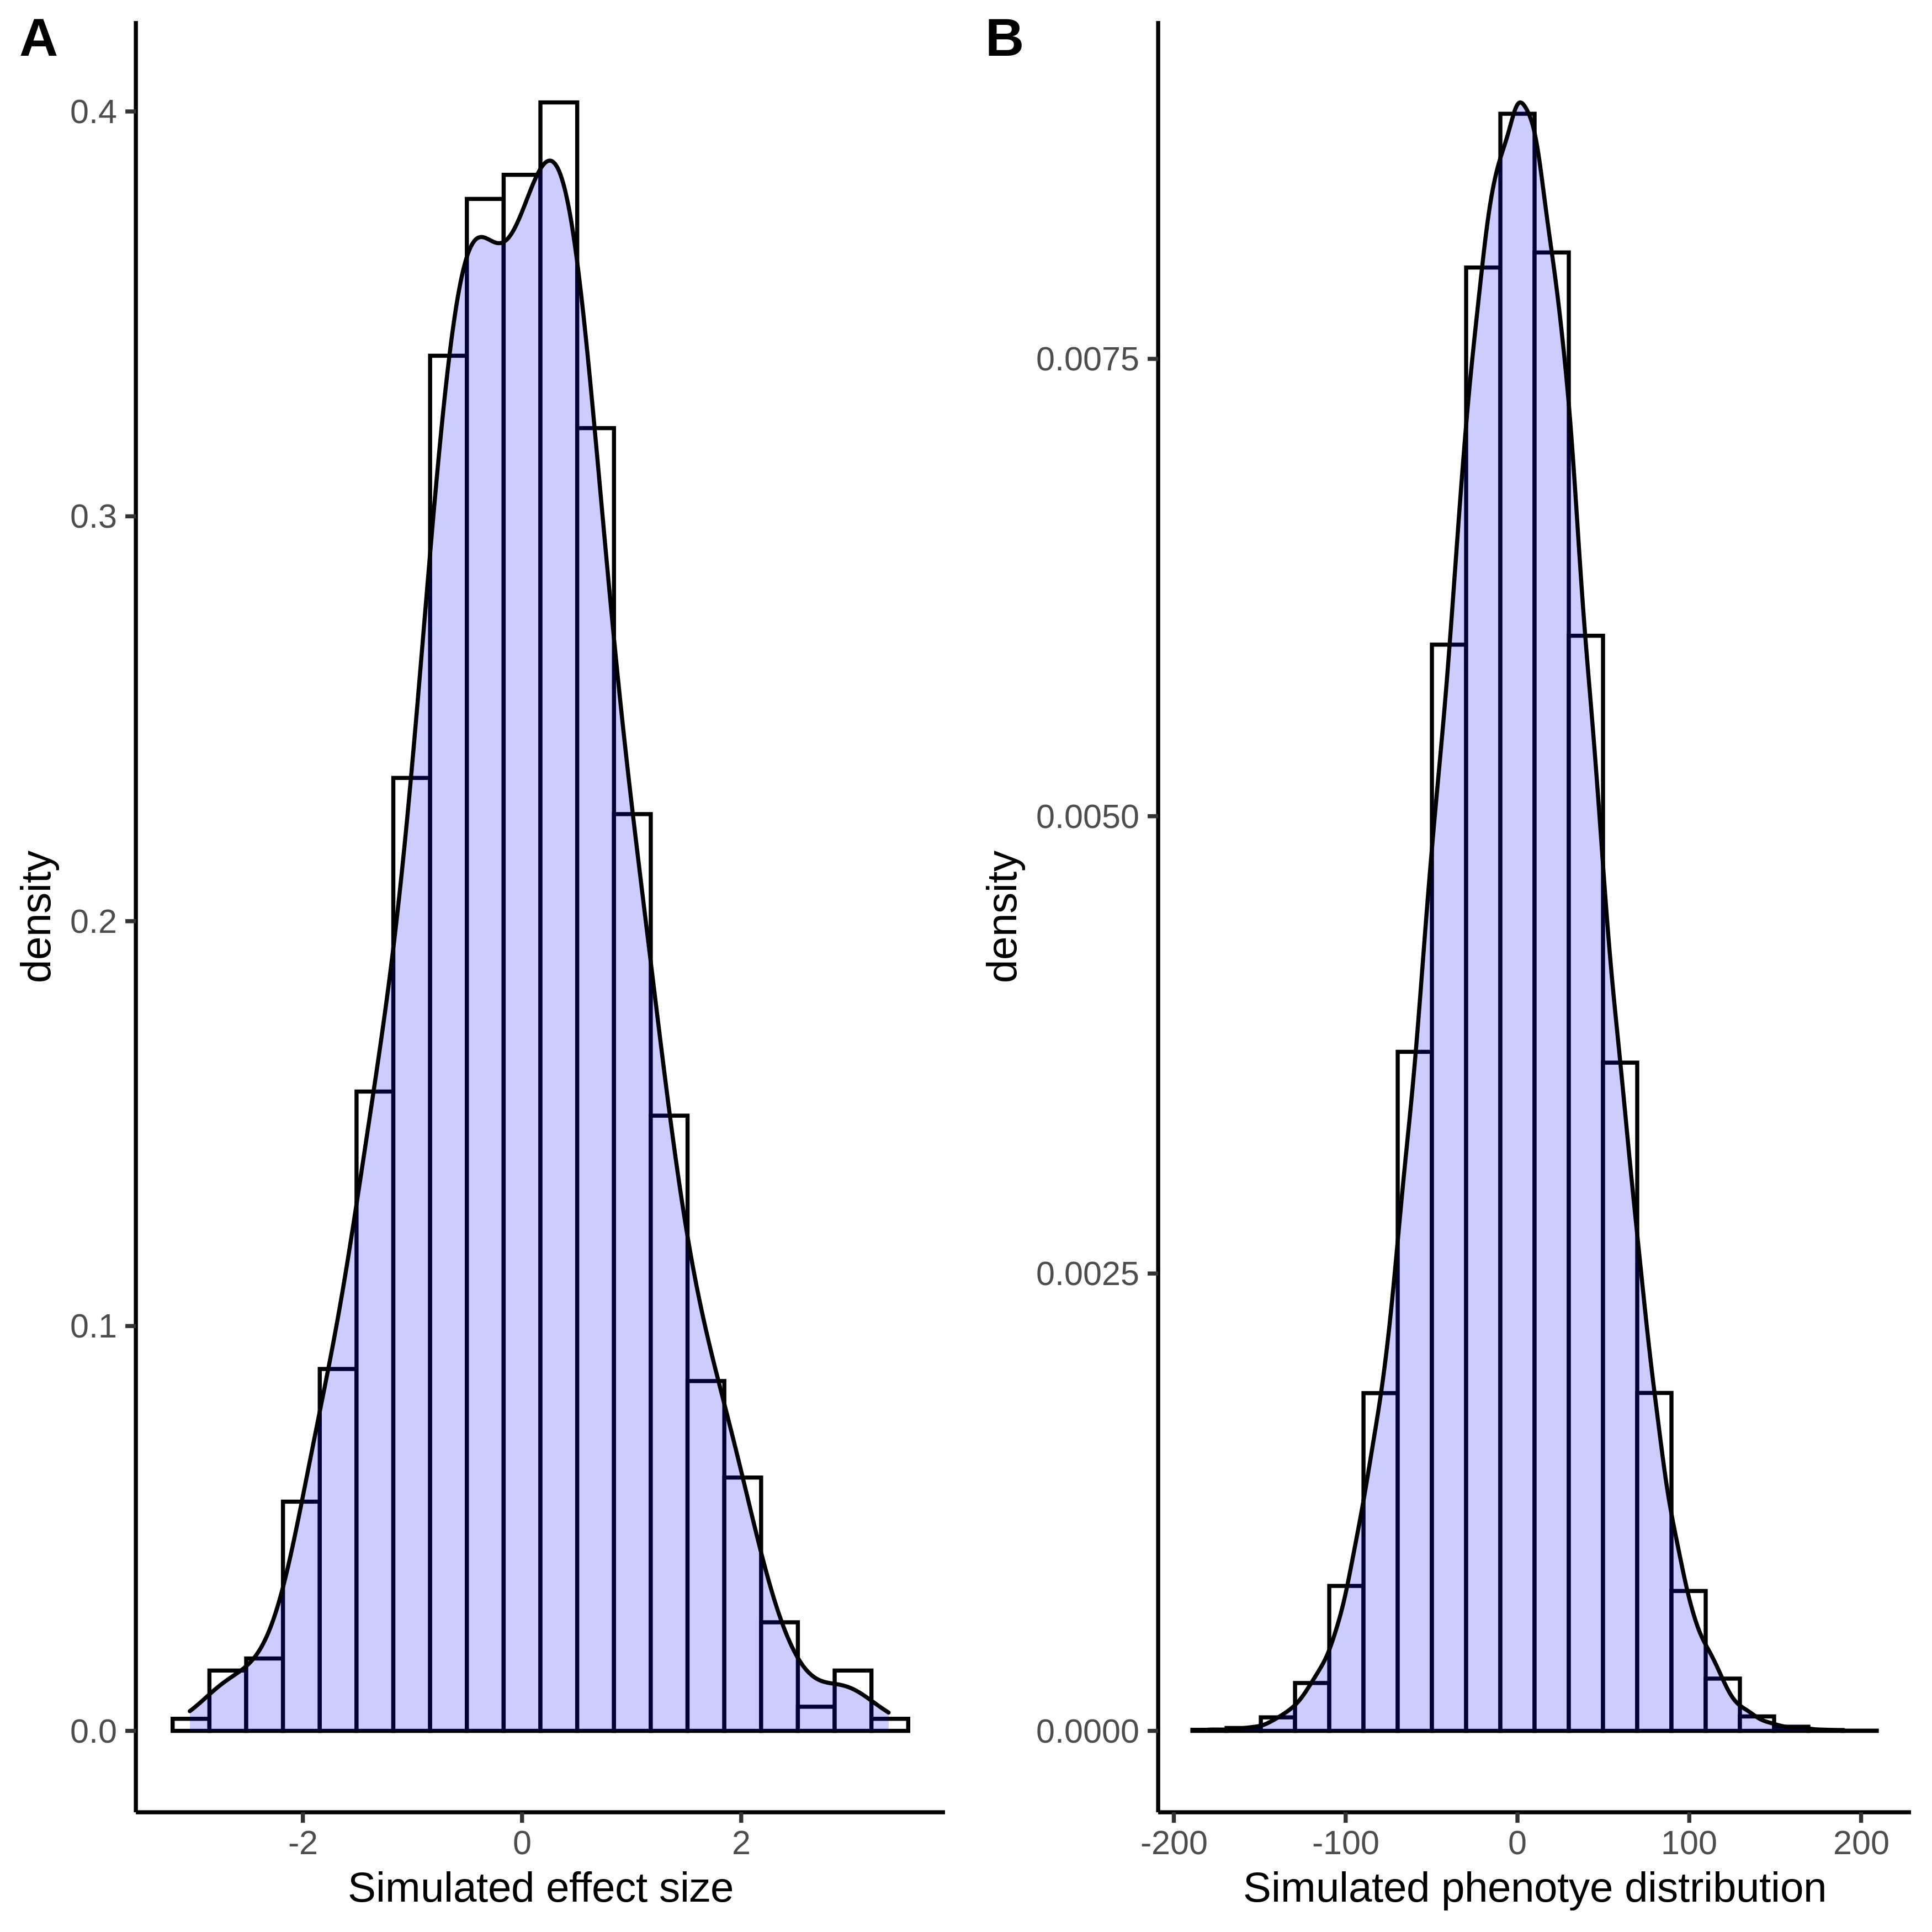
\includegraphics[width=\textwidth]{images/suppFig7.png}
  \caption{Simulation effect size and phenotype distribution. (A) Effect size distribution for 1000 causal loci with a SNP heritability of 0.5. (B) Simulated phenotype distribution for 100,000 samples}
\end{figure}

\begin{table}[ht]
\renewcommand{\thetable}{S\arabic{table}}
\centering
\caption{Fishers exact test for expected number of variants in each minor allele frequency bin}
\resizebox{1.2\textwidth}{!}{\begin{tabular}{rlrrrrrlr}
  \hline
 Bin & fastGWA & fastGWA bin & fastGWA-PGS & fastGWA-PGS bin & OR & CI & P.value \\ 
  \hline
$<$1\% & 126210 & 1096 & 30682 & 650 & 2.4 & 2.209-2.693 & 5.9E-65 \\ 
1-5\% & 115763 & 11543 & 28598 & 2734 & 0.96 & 0.9175-1.002 & 0.06 \\ 
5-10\% & 111480 & 15826 & 27312 & 4020 &   1 & 0.9988-1.076 & 0.057 \\ 
10-20\% & 99667 & 27639 & 22969 & 8363 & 1.3 & 1.276-1.351 & 4.4E-77 \\ 
20-50\% & 56104 & 71202 & 15767 & 15565 & 0.78 & 0.7588-0.7974 & 6.2E-88 \\ 
   \hline
\end{tabular}}
\thispagestyle{empty}
\end{table}


\begin{table}[h!]
\vspace{-7.5em}%
\renewcommand{\thetable}{S\arabic{table}}
\centering
\caption{Gene-property analysis results}
\begin{tabular}{lrrrrr}
  \hline
Tissue & NGenes & Beta & Beta Std & Se & P \\ 
  \hline
Muscle Skeletal & 2049 & 0.021 & 0.038 & 0.011 & 0.025 \\ 
  Esophagus Muscularis & 2049 & 0.03 & 0.054 & 0.019 & 0.054 \\ 
  Artery Tibial  & 2049 & 0.022 & 0.043 & 0.014 & 0.06 \\ 
  Esophagus Gastroesophageal J.. & 2049 & 0.027 & 0.05 & 0.019 & 0.08 \\ 
  Colon Sigmoid & 2049 & 0.026 & 0.046 & 0.019 & 0.086 \\ 
  Artery Aorta  & 2049 & 0.02 & 0.037 & 0.015 & 0.09 \\ 
  Kidney Medulla & 2049 & 0.017 & 0.028 & 0.016 & 0.14 \\ 
  Cells Cultured fibroblasts & 2049 & 0.0092 & 0.018 & 0.01 & 0.18 \\ 
  Thyroid & 2049 & 0.014 & 0.025 & 0.016 & 0.19 \\ 
  Kidney Cortex & 2049 & 0.013 & 0.021 & 0.015 & 0.2 \\ 
  Uterus & 2049 & 0.014 & 0.026 & 0.017 & 0.21 \\ 
  Bladder  & 2049 & 0.015 & 0.027 & 0.021 & 0.24 \\ 
  Artery Coronary & 2049 & 0.01 & 0.019 & 0.018 & 0.28 \\ 
  Brain Frontal Cortex BA9 & 2049 & 0.0066 & 0.011 & 0.011 & 0.28 \\ 
  Heart Atrial Appendage & 2049 & 0.0082 & 0.013 & 0.016 & 0.31 \\ 
  Brain Hypothalamus & 2049 & 0.0055 & 0.0086 & 0.014 & 0.34 \\ 
  Brain Anterior cingulate cor... & 2049 & 0.0049 & 0.0079 & 0.012 & 0.34 \\ 
  Brain Cortex & 2049 & 0.0042 & 0.0069 & 0.012 & 0.36 \\ 
  Brain Hippocampus & 2049 & 0.0026 & 0.0041 & 0.013 & 0.42 \\ 
  Breast Mammary Tissue & 2049 & 0.0039 & 0.0069 & 0.021 & 0.43 \\ 
  Skin Sun Exposed Lower leg & 2049 & 0.0027 & 0.0048 & 0.015 & 0.43 \\ 
  Skin Not Sun Exposed Suprapu... & 2049 & 0.0024 & 0.0042 & 0.015 & 0.44 \\ 
  Adipose Subcutaneous & 2049 & 0.0019 & 0.0035 & 0.017 & 0.46 \\ 
  Vagina  & 2049 & 0.0017 & 0.0029 & 0.019 & 0.47 \\ 
  Nerve Tibial  & 2049 & 0.0012 & 0.0021 & 0.016 & 0.47 \\ 
  Pituitary  & 2049 & -0.0001 & -0.0002 & 0.014 & 0.5 \\ 
  Brain Amygdala & 2049 & -0.0003 & -0.0005 & 0.013 & 0.51 \\ 
  Adrenal Gland & 2049 & -0.001 & -0.0017 & 0.016 & 0.52 \\ 
  Brain Nucleus accumbens basa... & 2049 & -0.0008 & -0.0013 & 0.013 & 0.53 \\ 
  Cervix Ectocervix & 2049 & -0.0024 & -0.0043 & 0.019 & 0.55 \\ 
  Testis  & 2049 & -0.0015 & -0.0023 & 0.01 & 0.56 \\ 
  Stomach  & 2049 & -0.0031 & -0.0052 & 0.02 & 0.56 \\ 
  Brain Substantia nigra & 2049 & -0.0021 & -0.0034 & 0.014 & 0.56 \\ 
  Brain Spinal cord cervical c... & 2049 & -0.003 & -0.0048 & 0.014 & 0.59 \\ 
  Liver & 2049 & -0.0026 & -0.0044 & 0.01 & 0.6 \\ 
  Adipose Visceral Omentum & 2049 & -0.0048 & -0.0087 & 0.018 & 0.61 \\ 
  Lung & 2049 & -0.0057 & -0.01 & 0.016 & 0.64 \\ 
  Minor Salivary Gland & 2049 & -0.0069 & -0.012 & 0.018 & 0.65 \\ 
  Brain Caudate basal ganglia & 2049 & -0.0051 & -0.008 & 0.013 & 0.65 \\ 
  Pancreas & 2049 & -0.0059 & -0.0091 & 0.014 & 0.66 \\ 
  Colon Transverse & 2049 & -0.0087 & -0.015 & 0.02 & 0.67 \\ 
  Whole Blood & 2049 & -0.004 & -0.007 & 0.0089 & 0.67 \\ 
  Esophagus Mucosa & 2049 & -0.0062 & -0.011 & 0.014 & 0.68 \\ 
  Brain Putamen basal ganglia & 2049 & -0.0066 & -0.01 & 0.013 & 0.69 \\ 
  Cervix Endocervix & 2049 & -0.0097 & -0.017 & 0.019 & 0.7 \\ 
  Ovary & 2049 & -0.0089 & -0.016 & 0.015 & 0.72 \\ 
  Heart Left Ventricle & 2049 & -0.013 & -0.02 & 0.015 & 0.8 \\ 
  Prostate & 2049 & -0.018 & -0.03 & 0.021 & 0.81 \\ 
  Brain Cerebellar Hemisphere & 2049 & -0.0095 & -0.018 & 0.0093 & 0.85 \\ 
  Brain Cerebellum & 2049 & -0.011 & -0.02 & 0.0097 & 0.86 \\ 
  Fallopian Tube & 2049 & -0.024 & -0.042 & 0.02 & 0.89 \\ 
  Small Intestine Terminal Ile... & 2049 & -0.024 & -0.04 & 0.018 & 0.91 \\ 
  Cells EBV-transformed lympho... & 2049 & -0.011 & -0.024 & 0.0072 & 0.94 \\ 
  Spleen & 2049 & -0.021 & -0.038 & 0.013 & 0.95 \\ 
   \hline
\end{tabular}
\thispagestyle{empty}
\end{table}

\begin{table}[h!]
\renewcommand{\thetable}{S\arabic{table}}
\centering
\tiny
\caption{Prediction of height using 74,000 most significant independent loci and the corresponding intersecting set of variants for each method}
\resizebox{.65\textwidth}{!}{\begin{tabular}{rlrr}
  \hline
Method & $R^2$ & se \\ 
  \hline
  \textbf{Top 74,000 variants}\\
fastGWA & 0.1296 & 0.0021 \\ 
  fastGWA-PGS & 0.1385 & 0.0022 \\ 
   \hline

   \textbf{37,514 intersecting variants} \\
fastGWA & 0.1177 & 0.0021\\ 
  fastGWA-PGS & 0.1192 & 0.0021 \\ 
   \hline
\end{tabular}}
\thispagestyle{empty}
\end{table}

\end{document}